\documentclass[
  bibliography=totoc,     % Literatur im Inhaltsverzeichnis
  captions=tableheading,  % Tabellenüberschriften
  titlepage=firstiscover, % Titelseite ist Deckblatt
]{scrartcl}

% Paket float verbessern
\usepackage{scrhack}

% Warnung, falls nochmal kompiliert werden muss
\usepackage[aux]{rerunfilecheck}

% unverzichtbare Mathe-Befehle
\usepackage{amsmath}
% viele Mathe-Symbole
\usepackage{amssymb}
% Erweiterungen für amsmath
\usepackage{mathtools}

% Fonteinstellungen
\usepackage{fontspec}
% Latin Modern Fonts werden automatisch geladen
% Alternativ zum Beispiel:
%\setromanfont{Libertinus Serif}
%\setsansfont{Libertinus Sans}
%\setmonofont{Libertinus Mono}

% Wenn man andere Schriftarten gesetzt hat,
% sollte man das Seiten-Layout neu berechnen lassen
\recalctypearea{}

% deutsche Spracheinstellungen
\usepackage{polyglossia}
\setmainlanguage{german}


\usepackage[
  math-style=ISO,    % ┐
  bold-style=ISO,    % │
  sans-style=italic, % │ ISO-Standard folgen
  nabla=upright,     % │
  partial=upright,   % ┘
  warnings-off={           % ┐
    mathtools-colon,       % │ unnötige Warnungen ausschalten
    mathtools-overbracket, % │
  },                       % ┘
]{unicode-math}

% traditionelle Fonts für Mathematik
\setmathfont{Latin Modern Math}
% Alternativ zum Beispiel:
%\setmathfont{Libertinus Math}

\setmathfont{XITS Math}[range={scr, bfscr}]
\setmathfont{XITS Math}[range={cal, bfcal}, StylisticSet=1]

% Zahlen und Einheiten
\usepackage[
  locale=DE,                   % deutsche Einstellungen
  separate-uncertainty=true,   % immer Fehler mit \pm
  per-mode=symbol-or-fraction, % / in inline math, fraction in display math
]{siunitx}

% chemische Formeln
\usepackage[
  version=4,
  math-greek=default, % ┐ mit unicode-math zusammenarbeiten
  text-greek=default, % ┘
]{mhchem}

% richtige Anführungszeichen
\usepackage[autostyle]{csquotes}

% schöne Brüche im Text
\usepackage{xfrac}

% Standardplatzierung für Floats einstellen
\usepackage{float}
\floatplacement{figure}{htbp}
\floatplacement{table}{htbp}

% Floats innerhalb einer Section halten
\usepackage[
  section, % Floats innerhalb der Section halten
  below,   % unterhalb der Section aber auf der selben Seite ist ok
]{placeins}

% Seite drehen für breite Tabellen: landscape Umgebung
\usepackage{pdflscape}

% Captions schöner machen.
\usepackage[
  labelfont=bf,        % Tabelle x: Abbildung y: ist jetzt fett
  font=small,          % Schrift etwas kleiner als Dokument
  width=0.9\textwidth, % maximale Breite einer Caption schmaler
]{caption}
% subfigure, subtable, subref
\usepackage{subcaption}

% Grafiken können eingebunden werden
\usepackage{graphicx}
% größere Variation von Dateinamen möglich
\usepackage{grffile}

% schöne Tabellen
\usepackage{booktabs}

% Verbesserungen am Schriftbild
\usepackage{microtype}

% Literaturverzeichnis
\usepackage[
  backend=biber,
]{biblatex}
% Quellendatenbank
\addbibresource{lit.bib}
\addbibresource{programme.bib}

% Hyperlinks im Dokument
\usepackage[
  unicode,        % Unicode in PDF-Attributen erlauben
  pdfusetitle,    % Titel, Autoren und Datum als PDF-Attribute
  pdfcreator={},  % ┐ PDF-Attribute säubern
  pdfproducer={}, % ┘
]{hyperref}
% erweiterte Bookmarks im PDF
\usepackage{bookmark}

% Trennung von Wörtern mit Strichen
\usepackage[shortcuts]{extdash}

\author{%
  Jan Philipp Jäkel\\%
  \href{mailto:jan.jaekel@tu-dortmund.de}{jan.jaekel@tu-dortmund.de}%
  \texorpdfstring{\and}{,}%
  Piet Hoffmann\\%
  \href{mailto:piet.hoffmann@tu-dortmund.de}{piet.hoffmann@tu-dortmund.de}%
}
\publishers{TU Dortmund – Fakultät Physik}

%\setmainfont{Comic Sans MS}

\subject{V701}
\title{Reichweite von \texorpdfstring{$\alpha$}{alpha}-Strahlung}

\date{
  \begin{align}
    \text{Durchführung: } & \text{22.5.2018} & \hspace{3em} & \text{Abgabe: 29.5.2018} \notag
%\\  \text{Korrektur: } & \text{29.5.2018} & \hspace {3em} & \notag
  \end{align}
}

%\date{%
%  Durchführung: DATUM
%  \hspace{3em}
%  Abgabe: DATUM
%}

\begin{document}

\maketitle
\thispagestyle{empty}
\tableofcontents
\newpage

\section{Theorie}
\label{sec:Theorie}
In diesem Versuch wird die Reichweite von $\alpha$-Strahlung in Luft untersucht.
Diese hängt mit der Energie der Strahlung zusammen, da die $\alpha$-Teilchen beim Durchlaufen von Materie über verschiedene Wechselwirkungen ihre diese abgeben.
Einerseits besteht die Möglichkeit, dass die Teilchen ihre Energie durch elastische Stöße bzw. Rutherford-Streuung abgeben, jedoch ist dies nicht der hauptsächliche Grund für die Energieabgabe.
Wesentlich bedeutender ist die Ionisation der Moleküle oder auch die Anregung und Aufteilung dieser. Diese Effekte lassen sich für hohe Energien über die Bethe-Bloch-Gleichung beschreiben:
\begin{equation}
	\label{bbgl}
	\symup{dE_\alpha} = -\frac{z^2e^4}{4\pi\epsilon_0m_e} \frac{nZ}{v^2} \ln\left(\frac{2m_ev^2}{I}\right) \symup{dx}
\end{equation}
Hierbei ist $z$ die Ladung und $v$ die Geschwindigkeit der $\alpha$-Teilchen, $I$ die Ionisierungsenergie, $Z$ die Ordnungszahl und $n$ die Teilchendichte der Luft.
Somit ist dieser Effekt direkt abhängig von der Energie der Strahlung und der Dichte der Luft.
Es lässt sich zudem eine Reichweite $R$ definieren:
\begin{equation}
	\label{R}
	R=-\int_0^{E_\alpha}\frac{\symup{dE_\alpha}}{\frac{\symup{dE_\alpha}}{dx}}
\end{equation}
\\
Für nierdige Energien verliert die Gleichung \eqref{bbgl} jedoch an Geltung. Deswegen wird aus empirisch gewonnenen Messergebnissen eine Gleichung für eine mittlere Reichweite $R_\text m$ bestimmt.
Die mittlere Reichweite wird definiert als den Abstand, bei welchem noch die Hälfte der $\alpha$-Teilchen vorhanden sind.
Es ergibt sich für $\alpha$-Strahlung in Luft mit Energien $E_\alpha \le \SI{2.5}{\mega\electronvolt}$:
\begin{equation}
	\label{Rm}
	R_\text m = E_\alpha^{3/2} \frac{\SI{3.1}{\milli\meter}}{\si{\mega\electronvolt}^{3/2}}
\end{equation}
Diese mittlere Reichweite ist in Gasen für konstantes Volumen und konstante Temperatur proportional zum Druck $p$.
Es lässt sich somit bei einer Messung mit variirendem Druck ein Rückschluss auf die Reichweite ziehen.
Hierfür ist es sinnvoll eine effektive Länge $x$ zwischen Quelle und Detektor zu definieren mit
\begin{equation}
	\label{xeff}
	x = x_0\frac{p}{p_0},
\end{equation}
wobei $x_0$ der tatsächliche Abstand zwischen Strahler und Detektor und $p_0 = \SI{1013}{\milli\bar}$ der Atmosphärendruck ist.

\section{Durchführung}
\label{sec:Durchführung}
Der Versuchsaufbau besteht aus einem mittels einer Vakuumpumpe evakuierbaren Glaszylinder. In diesem befindet sich ein Detektor in der Form eines Halbleitersperrschichtzählers und ein $\alpha$-STrahler, in 
diesem Fall ein \ce{^{241}_{95}Am} Präparat. Dieses zerfällt auf folgende Weise:
\begin{equation}
	\ce{^{241}_{95}Am -> ^{237}_{93}Np + ^4_2He^{++}}
\end{equation}
Die Probe ist so in dem Zylinder befestigt, dass ihr Abstand zum Detektor variiert werden kann.
Im Detektor werden durch die eintreffende Strahlung Elektron-Loch-Paare erzeugt, welche zu einem Stromimpuls proportional zur Energie des erzeugenden $\alpha$-Teilchens ist.
Der Detektor ist über einen Vorverstärker an einen Multi-Channel-Analyzer angeschlossen, welcher die am Detektor eingetroffene Strahlung in Energiekanäle einordnet und dies an einen Computer weitergibt.
Der Aufbau ist in Abbildung \ref{fig:aufbau} abgebildet.
\begin{figure}[H]
  \centering
  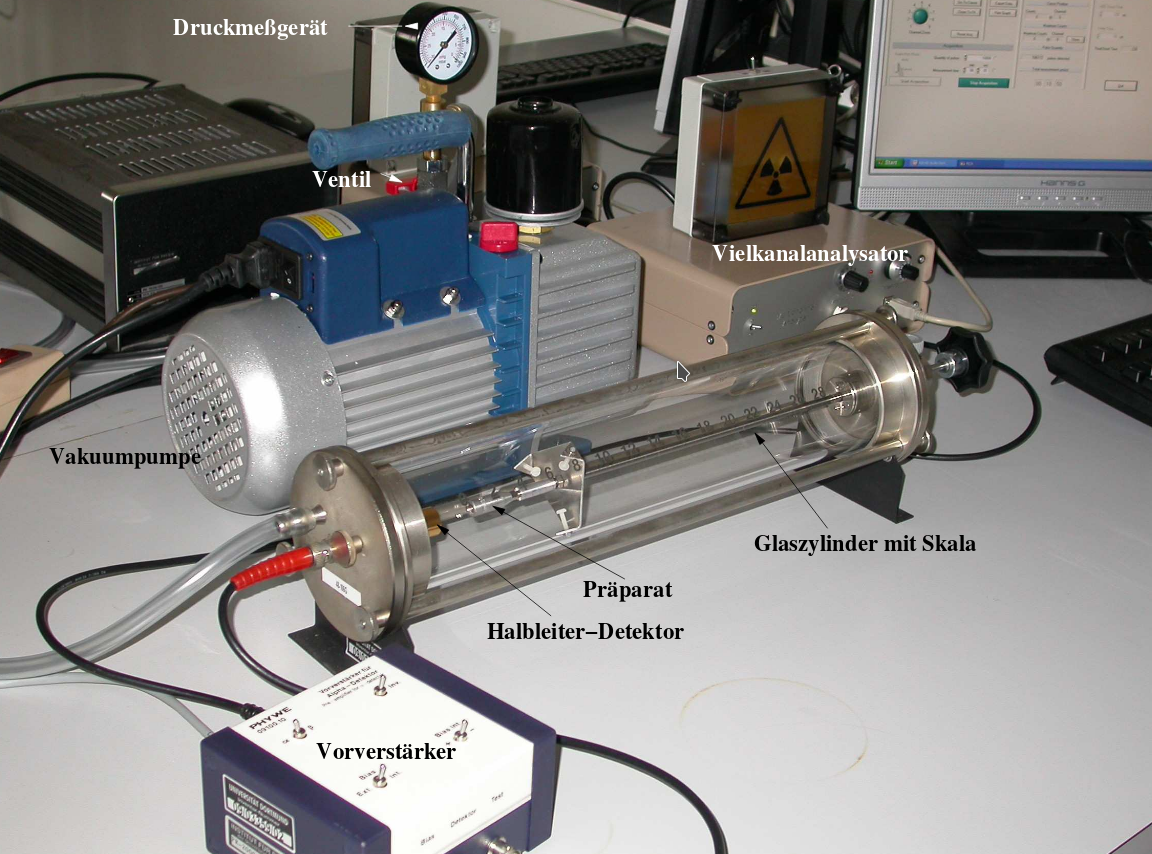
\includegraphics[width=\textwidth]{content/aufbau.png}
  \caption{Versuchsaufbau.}
  \label{fig:aufbau}
\end{figure}
\noindent
Um den Multi-Channel-Analyzer einzurichten muss zunächst über die Diskreminatorschwelle die Hintergundstrahlung herausgefiltert werden. Dazu wird die Schwelle bei nicht evakuiertem Zylinder und großem 
Abstand zwischen Probe und Detektor so weit nachjustiert, bis keine Events mehr registriert werden. Anschließend wird die Probe so weit herangefahren, dass wieder Impulse registriert werden.
\subsection{Bestimmung der Reichweite von \texorpdfstring{$\alpha$}{alpha}-Strahlung}
Für die Bestimmung der Reichweite der Strahlung wird der Zylinder evakuiert, bis das Manometer der Vakuumpumpe einen Druck $p \approx \SI{0}{\milli\bar}$ innerhalb des Zylinders anzeigt.
Nun wird die Energieverteilung der eintreffenden Strahlung in Abhängigkeit vom Druck bestimmt, der nach jeder Messung um $\SI{50}{\milli\bar}$ erhöht wird, bis der Atmosphärendruck wieder erreicht ist.
Dabei wird für jede Messung über $\SI{120}{\second}$ gemessen und die Position des Energiemaximums, sowie die Gesamtzahl der eingenangenen Events notiert. Es wird für spätere Berechnugen angenommen, dass 
bei $p=0$ das Energiemaximum einem Wert von $\SI{4}{\mega\electronvolt}$ entspricht und die 
Skala des Multi-Channel-Analyzers linear ist.
\subsection{Statistik des radioaktiven Zerfalls}
Um zu überprüfen, ob die Statistik des radioaktiven Zerfalls tatsächlich nach der Piossonverteilung geschieht, werden die Events bei evakuierten Zylinder gezählt.
Um eine Aussage über die Statistik treffen zu können wird \num{100} mal über eine Dauer von \SI{10}{\second} gemessen. Die erhaltenen Zählraten werden mit einer Gauß- sowie einer Poissonverteilung 
verglichen. Dafür wird der Mittelwert und die Varianz der Messwerte bestimmt.

\section{Auswertung}
\label{sec:Auswertung}

Es werden zwei Messungen für zwei verschiedene feste Abstände durchgeführt.
Es werden Zählrate, Drücke und Channel aufgenommen.
Der Channel für die Messung bei $0\si{\milli\bar}$ entspricht $4\si{\mega\electronvolt}$.
Die effektive Länge wird mit Gleichung bestimmt.
Die so erhaltenen Werte sind in Tabelle\ref{tab:mess1} aufgetragen.
\begin{table}[H]
    \caption{Messwerte für einen festen Abstand von $x_0=2\si{\centi\meter}$.}
    \label{tab:mess1}
    \centering
    \begin{tabular}{S[table-format=4.0] S[table-format=1.2(0)e0] S[table-format=4.0(0)e0] S[table-format=2.2(0)e0]  }
        \toprule
        {Zählrate$1/120s$} & {Energie$/\si{\mega\electronvolt}$} & {Druck$/\si{\milli\bar}$} &{effektive Länge$\si{\centi\meter}$} \\
        \midrule
        74271 & 4.00 & 0 & 0.00\\
        73634 & 3.97 & 50 & 0.10\\
        71805 & 3.87 & 100 & 0.20\\
        69331 & 3.78 & 150 & 0.30\\
        67027 & 3.60 & 200 & 0.39\\
        64835 & 3.55 & 250 & 0.49\\
        61440 & 3.43 & 300 & 0.59\\
        33760 & 3.06 & 350 & 0.69\\
        28770 & 3.02 & 400 & 0.79\\
        41401 & 3.06 & 450 & 0.89\\
        41124 & 3.05 & 500 & 0.99\\
        33198 & 3.01 & 550 & 1.09\\
        27967 & 3.02 & 600 & 1.18\\
        20681 & 3.00 & 650 & 1.28\\
        15966 & 2.99 & 700 & 1.38\\
        9472 & 2.99 & 750 & 1.48\\
        6076 & 2.99 & 800 & 1.58\\
        2561 & 3.01 & 850 & 1.68\\
        937 & 2.99 & 900 & 1.78\\
        397 & 2.98 & 950 & 1.88\\
        99 & 3.00 & 1000 & 1.97\\

        \bottomrule
    \end{tabular}
\end{table}
\noindent Die Zählrate wird in Abbildung\ref{fig:c1} gegen die effektive Länge aufgetragen.
Es wird eine Reggressionsgerade mit SciPy/Python nach der Funktionsvorschrift
\begin{equation*}
  f(x) = mx +b
\end{equation*}
erstellt.
\begin{figure}[H]
  \centering
  \includegraphics{build/counts1.pdf}
  \caption{Lineare Reggression für die Zählrate in Abhängigkeit der effektiven Länge.}
  \label{fig:c1}
\end{figure}
\noindent Dabei ergeben sich folgenede Parameter:
\begin{equation*}
  m =(-384\pm29)\si{\per\centi\meter}
\end{equation*}
und
\begin{equation*}
  b =667\pm27  .
\end{equation*}
Die mittlere Reichweite ergibt sich dann als Schnittpunkt der Regressionsgeraden mit der Horizontalen bei $y=309.46$.
Die mittlere Reichweite kann, dann durch umstellen der Funktionsvorschrift, mit
\begin{equation*}
  R_m=\frac{309.46-b}{m}
\end{equation*}
bestimmt werden.
Der Fehler der mittleren Reichweite wird mit Gaußscher Fehlerfortpflanzung nach
\begin{equation*}
  \sigma_R = \sqrt{(\frac{b-309.46}{m^2}\sigma_m)^2 +(-\frac{1}{m}\sigma_b)^2}
\end{equation*}
berrechnet.
Der so erhaltene Wert beträgt $R_m= (0.93\pm0.1)\si{\centi\meter}$.
Damit lässt sich nach Gleichung eine Energie von $E_{\alpha} = 0.45\si{\mega\electronvolt}$ bestimmen.
Die Energie wird in Abbildung\ref{fig:e1} als Funktion der effektiven Länge aufgetragen.
Es wird eine Reggressionsgerade nach der Vorschrift
\begin{equation*}
  f(x) = mx + b
\end{equation*}
durch die Messwerte gezogen.
Für die Reggressionsrechnung wird nur der lineare Anteil der Messwerte verwendet.
\begin{figure}[H]
  \centering
  \includegraphics{build/energie1.pdf}
  \caption{Lineare Reggression für die Energie in Abhängigkeit der effektiven Länge.}
  \label{fig:e1}
\end{figure}
\noindent Der Energieverlust $-\frac{dE}{dx}$ kann dann als Steigung der Regression bestimmt werden.
Damit ergibt sich ein Energieverlust von
\begin{equation*}
  -\frac{dE}{dx} =(-0.52\pm0.07)\si{\mega\electronvolt\per\centi\meter} .
\end{equation*}
Analog wird für den zweiten Abstand vorgegangen.
Die Messwerte sind in Tabelle \ref{tab:mess2} aufgetragen
\begin{table}[H]
    \caption{Messwerte für einen festen Abstand von $x_0=1.5\si{\centi\meter}$.}
    \label{tab:mess2}
    \centering
    \begin{tabular}{S[table-format=4.0] S[table-format=1.2(0)e0] S[table-format=4.0(0)e0] S[table-format=2.2(0)e0]  }
        \toprule
        {Zählrate$1/120s$} & {Energie$/\si{\mega\electronvolt}$} & {Druck$/\si{\milli\bar}$} &{effektive Länge$\si{\centi\meter}$} \\
        \midrule
        148139 & 4.00 & 0 & 0.00\\
        150632 & 3.93 & 50 & 0.07\\
        149256 & 3.85 & 100 & 0.15\\
        143513 & 3.56 & 150 & 0.22\\
        139419 & 3.46 & 200 & 0.30\\
        145173 & 3.56 & 250 & 0.37\\
        136922 & 3.29 & 300 & 0.44\\
        134960 & 3.20 & 350 & 0.52\\
        133809 & 3.15 & 400 & 0.59\\
        138624 & 3.22 & 450 & 0.66\\
        138244 & 3.19 & 500 & 0.74\\
        130125 & 2.95 & 550 & 0.81\\
        131421 & 2.95 & 600 & 0.89\\
        125958 & 2.79 & 650 & 0.96\\
        123717 & 2.72 & 700 & 1.04\\
        121739 & 2.67 & 750 & 1.11\\
        120083 & 2.59 & 800 & 1.18\\
        117426 & 2.49 & 850 & 1.26\\
        114320 & 2.45 & 900 & 1.33\\
        112018 & 2.42 & 950 & 1.41\\
        104394 & 2.36 & 1000 & 1.48\\
        \bottomrule
    \end{tabular}
\end{table}

\section{Diskussion}
\label{sec:Diskussion}


\nocite{*}
\printbibliography{}

\end{document}
